\section{Scanned Synthesis Matrix
Editor}\label{scannedSynthesisMatrixEditor}

Scanned Synthesis Matrix Editor

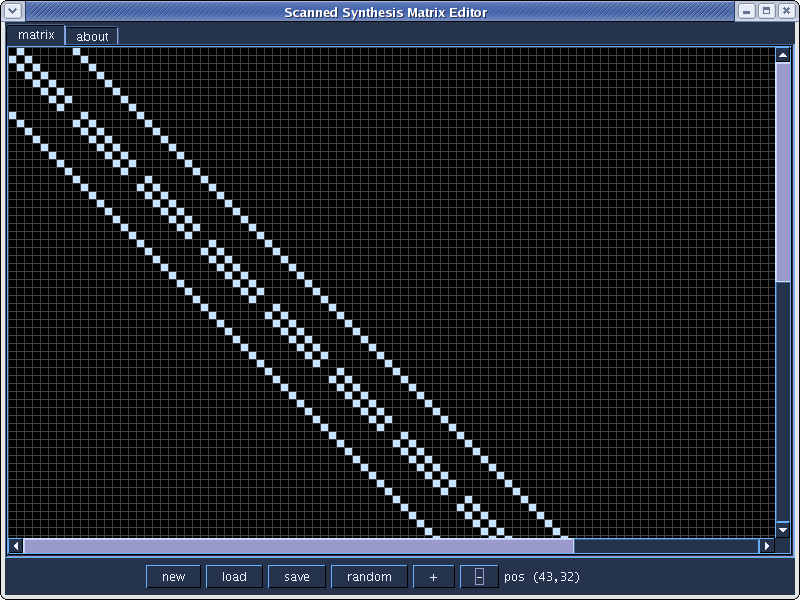
\includegraphics{images/scannedSynthesisMatrixEditor.png}

The Scanned Synthesis Matrix Editor tools allows for editing and
creating matrix files used by the Scanned Synthesis opcodes in Csound.

\begin{itemize}
\tightlist
\item
  Using "New" will ask what size matrix to create.
\item
  For editing, click anywhere on the matrix. This will either turn on or
  turn off that square, setting the connection between the masses to
  either 1 or 0.
\item
  After editing, press "Save" to save out the matrix to a file.
\item
  You can also click the "Random" button to create a randomized matrix.
\end{itemize}
